\documentclass[a4paper,12pt]{article}

\usepackage{cmap}					
\usepackage[T2A]{fontenc}			
\usepackage[utf8]{inputenc}			
\usepackage[english,russian]{babel}	

\usepackage{amsmath,amsfonts,amssymb,amsthm,mathtools} 
\usepackage{wasysym}


\usepackage{graphicx}
%\usepackage[cache=false]{minted}

\usepackage{indentfirst}
\usepackage{amssymb}


\usepackage{listings} 
\lstset{
	numbers = left,
	frame = single
}
\usepackage{fancyvrb}
%\DefineShortVerb{\|}

\usepackage{color}
\usepackage{caption}
\DeclareCaptionFont{white}{\color{black}}
\DeclareCaptionFormat{listing}{\colorbox{white}{\parbox{\textwidth}{#1#2#3}}}
\captionsetup[lstlisting]{format=listing,labelfont=white,textfont=white}


\usepackage{listings}

\usepackage{geometry}
\geometry{left=2cm}
\geometry{right=1.5cm}
\geometry{top=1cm}
\geometry{bottom=2cm}
\setlength{\parindent}{5ex}
\setlength{\parskip}{0.5em}

\begin{document}

% Титульный лист
\large
\begin{center}
Федеральное государственное бюджетное образовательное учреждение 
высшего образования <<Московский государственный технический 
университет имени Н. Э. Баумана>> 
(национальный исследовательский университет)
\end{center}

\vspace*{30mm} 

\LARGE
\begin{center}
Дисциплина: <<Анализ алгоритмов>>

Отчет по лабораторной работе №5
\end{center}

\vspace*{30mm} 

\huge
\begin{center}
Тема работы:\\
<<Конвейерная обработка данных>>
\end{center}
\vspace*{30mm} 

\large
\begin{flushright}
Студент: Аминов Т. С. \\
Группа: ИУ7-55Б \\
Преподаватели: Волкова Л. Л., \\ Строганов Ю. В. \\
\end{flushright}

\vspace*{40mm}
\begin{center}
Москва, 2019 г.  
\end{center}
\thispagestyle{empty}




\tableofcontents
% \setcounter{page}{1}

\newpage

\section*{Введение}
\addcontentsline{toc}{section}{Введение}

Имеется большое количество важных задач, решение которых требует использования огромных вычислительных мощностей, зачастую недоступных для современных 
вычислительных систем.

Параллелизм может значительно ускорить решение
таких задач. Особое место среди систем подобного рода занимает
конвейерный обработчик. Он прост для понимания,
ведь принцип его работы основан на реальном механизме
непрерыного действия. ~\cite{voev}

\textbf{Цель лабораторной работы:} получить навык организации асинхронной передачи 
данных между потоками на примере конвейерной обработки информации

\textbf{Задачи работы:}
	
\begin{enumerate} 
\item[1)] изучить алгоритм конвейеризации и алгоритм шифрования RSA;
\item[2)] реализовать конвейерную систему шифрования/дешифрования алгоритмом RSA;
\item[3)] провести журналирование событий в конвейерной обработке;
\item[4)] описать и обосновать полученные результаты в отчете о лабораторной 
работе, выполненного как расчётно-пояснительная записка. 
\end{enumerate} 
\pagebreak

\section{Аналитический раздел}
	
В данном разделе будет рассмотрены алгоритм конвейеризации и алгоритм шифрования RSA.
	
\subsection{Описание алгоритмов}

\subsubsection{Алгоритм конвейерной обработки данных}

Конвейеризация --- это техника, в результате которой  задача
разбивается  на некоторое число подзадач,
которые  выполняются последовательно.
Конвейерный подход позволяет создавать эффективные параллельные реализации обычных 
неспециализированных алгоритмов \cite{iu7}.

Каждая  подкоманда   выполняется на своем логическом  устройстве.
Все     логические    устройства   (ступени)  соединяются последовательно
таким образом, что выход  $i$-ой   ступени   связан   с   
входом   ($i+1$)-ой   ступени,  все ступени  работают  одновременно.  
Множество  ступеней называется    конвейером.    
Выигрыш     во    времени достигается при  выполнении  нескольких задач  
за  счет параллельной   работы   ступеней,  
вовлекая  на  каждом такте новую задачу или команду  \cite{korn}.

Каждое звено конвейера выполняет следующие действия:

\begin{itemize}
\item     получить данные,

\item     обработать данные,

\item      послать данные следующим звеньям.
\end{itemize}

\subsubsection{Алгоритм шифрования RSA}
RSA (аббревиатура от фамилий Rivest, Shamir и Adleman) — криптографический алгоритм с открытым ключом, основывающийся на вычислительной сложности задачи факторизации больших целых чисел \cite{rsa_opr}.

Алгоритм находит пары чисел $(e, n) $ и $(d, n) $, являющиеся открытым и закрытым ключом соответственно. Открытым ключом зашифровывают сообщение, а закрытым – расшифровывают. Пара чисел закрытого ключа держится в секрете
\cite{rsa_opr}.

Шифруемый символ представляют в виде числа – его номера в алфавите или кода в таблице символов (например ASCII или Unicode).

Шифрование производится по формуле:
\[
	 C_i = M^e_i \: mod \: n,
\]
где $(e, n) $ - открытый ключ, $M_i$ - шифруемый символ, $C_i$ - зашифрованный символ. 

Расшифровка сообщения производится по формуле:
\[
	 M_i = C^d_i \: mod \: n,
\] 
где $(d, n) $ - закрытый ключ, $M_i$ - расшифрованный символ, $C_i$ - зашифрованный символ. \cite{rsa_alg}.
\subsection*{Выводы}
\addcontentsline{toc}{subsection}{Выводы}

Рассмотрены алгоритм конвейерной обработки данных и алгоритм шифрования RSA, выделены их ключевые моменты. 
\newpage

\section{Конструкторский раздел}

В разделе приводятся схемы алгоритма конвейерной обработки данных и алгоритма RSA.

\subsection{Разработка алгоритмов}

На рис. \ref{fig:insert} приведена схема 
общая схема конвейерной обработки.
        
\begin{figure}[h!]
\begin{center}
{\includegraphics[width=\textwidth]{img/conv.jpg}}
\caption{
Схема работы конвейера}
\label{fig:insert}
\end{center}
\end{figure}

Псевдокод главной функции:

\begin{flushleft}
\texttt{1. Создать 3 потока, мьютекса и очереди\\
2. Заполнить массив объектов значениями от 1 до n\\
3. Добавить элементы массива в очередь 1\\
4. Применить join ко всем потокам\\
5. Записать информации из массива результатов в лог-файл\\
}
\end{flushleft}

Псевдокод для ленты 1:

\begin{flushleft}
\texttt{1. Бесконечный цикл\\
2. \hspace{1.5cm} Заблокировать мьютекс 1\\
3. \hspace{1.5cm} Если очередь 1 не пуста\\
4. \hspace{3cm} Извлечь элемент из очереди\\
5. \hspace{3cm} Записать информацию о начале работы\\
6. \hspace{3cm} Добавить элемент в результирующий массив\\
7. \hspace{3cm} Выполнить функции 1\\
8. \hspace{3cm} Добавить элемент в очередь 2\\
8. \hspace{3cm} Записать информацию об окончании работы\\
10. \hspace{3cm} Добавить элемент в результирующий массив\\
11. \hspace{3cm} Если элемент равен n\\
12. \hspace{4.5cm} Завершить работу\\
13. \hspace{1.5cm} Разблокировать мьютекс 1\\
}
\end{flushleft}

Псевдокод для ленты 2:

\begin{flushleft}
\texttt{1. Бесконечный цикл\\
2. \hspace{1.5cm} Заблокировать мьютекс 2\\
3. \hspace{1.5cm} Если очередь 2 не пуста\\
4. \hspace{3cm} Извлечь элемент из очереди\\
5. \hspace{3cm} Записать информацию о начале работы\\
6. \hspace{3cm} Добавить элемент в результирующий массив\\
7. \hspace{3cm} Выполнить функции 2\\
8. \hspace{3cm} Добавить элемент в очередь 3\\
9. \hspace{3cm} Записать информацию об окончании работы\\
10. \hspace{3cm} Добавить элемент в результирующий массив\\
11. \hspace{3cm} Если элемент равен n\\
12. \hspace{4.5cm} Завершить работу\\
13. \hspace{1.5cm} Разблокировать мьютекс 2\\
}
\end{flushleft}

Псевдокод для ленты 3:

\begin{flushleft}
\texttt{1. Бесконечный цикл\\
2. \hspace{1.5cm} Заблокировать мьютекс 3\\
3. \hspace{1.5cm} Если очередь 3 не пуста\\
4. \hspace{3cm} Извлечь элемент из очереди\\
5. \hspace{3cm} Записать информацию о начале работы\\
6. \hspace{3cm} Добавить элемент в результирующий массив\\
7. \hspace{3cm} Выполнить функции 3\\
8. \hspace{3cm} Записать информацию об окончании работы\\
9. \hspace{3cm} Добавить элемент в результирующий массив\\
10. \hspace{3cm} Если элемент равен n\\
11. \hspace{4.5cm} Завершить работу\\
12. \hspace{1.5cm} Разблокировать мьютекс 3\\
}
\end{flushleft}
\newpage
На рисунках \ref{fig:s1}, \ref{fig:s2} и \ref{fig:s3}  приведены схемы алгоритма RSA, разбитые на этапы для конвейера.

\begin{figure}[h!]
    \begin{center}
    		{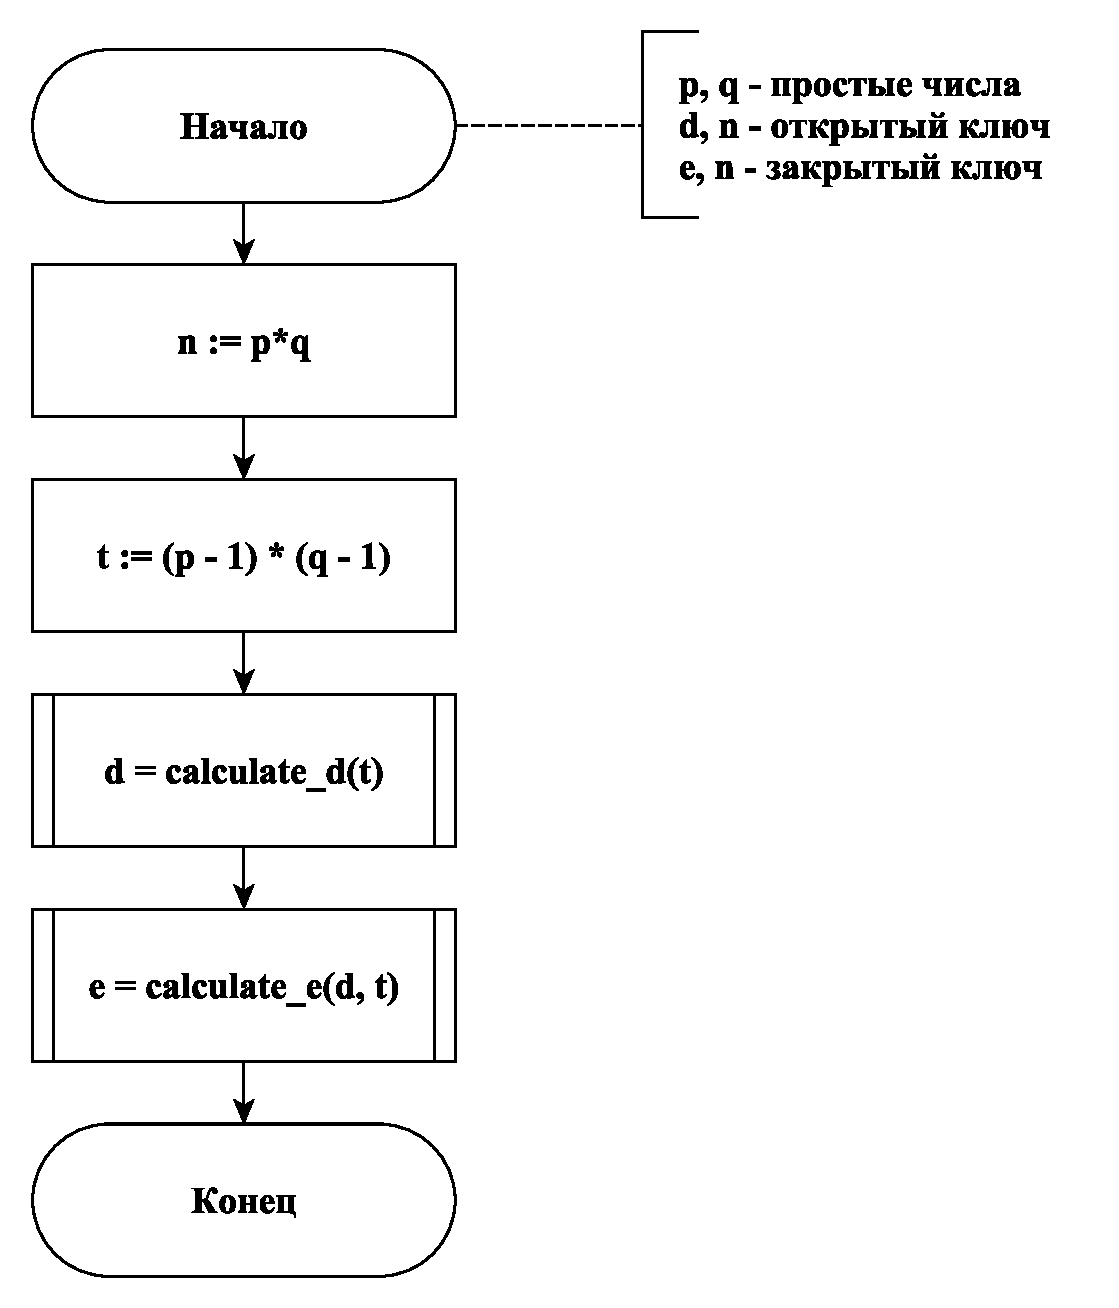
\includegraphics[scale = 0.5]{diagram/rsa1.pdf}}
       		\caption{Схема алгоритма генерации ключей }
       		\label{fig:s1}
	\end{center}
\end{figure}

\begin{figure}[h!]
    \begin{center}
    		{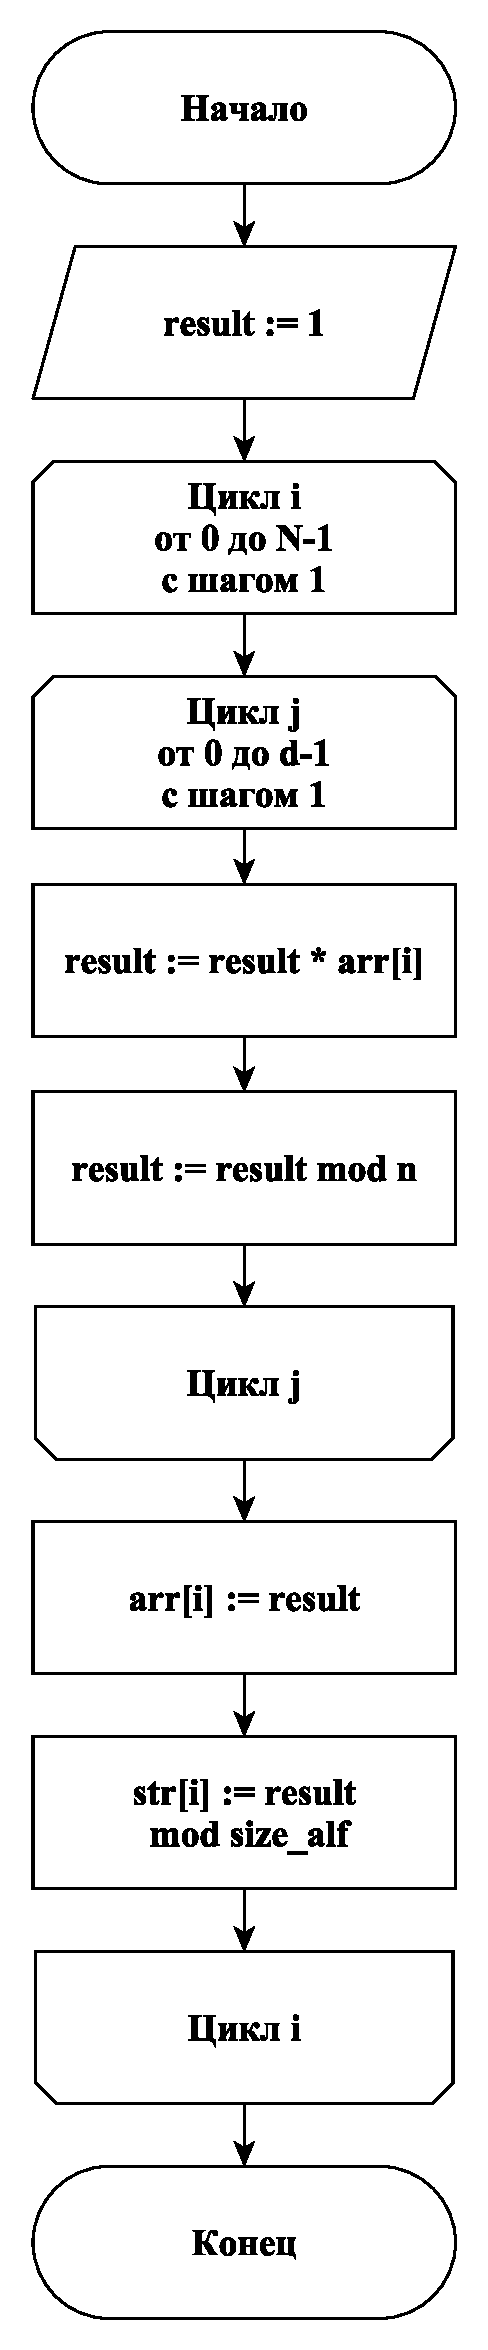
\includegraphics[scale = 0.5]{diagram/rsa2.pdf}}
       		\caption{Схема алгоритма шифрования строки }
       		\label{fig:s2}
	\end{center}
\end{figure}

\begin{figure}[h!]
    \begin{center}
    		{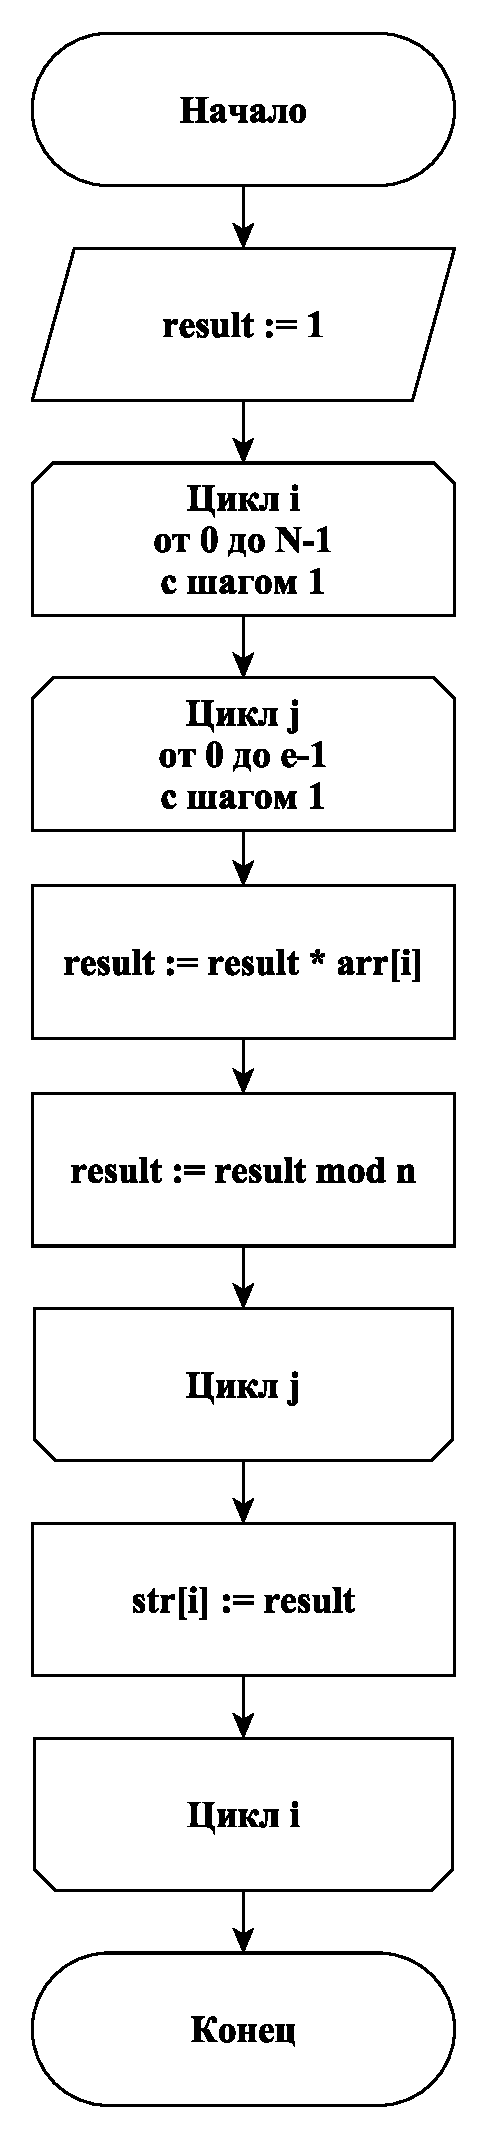
\includegraphics[scale = 0.5]{diagram/rsa3.pdf}}
       		\caption{Схема алгоритма дешифрования строки }
       		\label{fig:s3}
	\end{center}
\end{figure}
\newpage
	
	\mbox{}
	\newpage

\subsection*{Выводы}
\addcontentsline{toc}{subsection}{Выводы}

В разделе представлен псевдокод конвейерной обработки данных.
Даны интерпретации главной функции
и 3 функций, имитирующих работу лент.
\newpage

\section{Технологический раздел}

Здесь описываются требования к программному 
обеспечению и средства реализации, приводятся листинги 
программы.

\subsection{Требования к программному обеспечению}

\begin{flushleft}
Входные данные: 
	 \begin{enumerate} 
	 \item[1)] целое положительное число - количество строк для шифрования;
	 \item[2)] целое положительное число - максимальная длина строки;
	 \item[3)] строка - имя файла логов.
	 \end{enumerate}
	
	Выходные данные: файл с логами.

\end{flushleft}
	
На рис. \ref{fig:idef0} приведена 
функциональная схема 
конвейерной обработки данных.
        
\begin{figure}[h!]
\begin{center}
{\includegraphics[scale = 0.7]{img/idef0.jpg}}
\caption{Функциональная схема 
конвейерной обработки данных}
\label{fig:idef0}
\end{center}
\end{figure}
	
\subsection{Средства реализации}

Программа написана на языке С++, т. к. этот язык предоставляет программисту широкие возможности реализации самых разнообразных алгоритмов, обладает высокой эффективностью и значительным набором стандартных классов и процедур. В качестве среды разработки использовался  фреймворк QT 5.13.1.
	
Для хранения массива, строк применяются 
контейнерные классы \textit{std::vector}, \textit{std::string} из стандартной 
библиотеки шаблонов STL. Кроме того, для реализации конвейера
используются \textit{std::thread} и \textit{std::mutex}.
	
Замер времени
производится с помощью функции \textit{GetLocalTime} из библиотеки \textit{windows.h}.
    
\subsection{Листинг программы}

Реализация конвейерной обработки данных представлена на листингах \ref{lst0}-\ref{lst5}.

\begin{lstlisting}[label=lst0, caption={Структура объекта конвейера}]
struct Conv_obj {
    int index;
    std::string str;
    std::vector<long long int> vec;
    Key public_key, private_key;
};
\end{lstlisting}

\begin{lstlisting}[label=lst1,caption=Структура объекта для записи в файл логов]
struct File_obj {
    int index_str;
    int num_belt;
    SYSTEMTIME t;
    char state;
};
\end{lstlisting}
 
\begin{lstlisting}[label=lst2,caption=Главная функция конвейера]
void conveyor() {
    std::queue<Conv_obj> queue_1, queue_2, queue_3;
    std::vector<std::string> vec_str;
    std::vector<Conv_obj> vec_elem;
    vec_init(vec_str, MAX_ELEM, len_str);
    for (size_t i = 0; i < vec_str.size(); i++) {
        Conv_obj tmp;
        tmp.str = vec_str[i];
        tmp.index = i + 1;
        vec_elem.push_back(tmp);
    }

    for (size_t i = 0; i < vec_str.size(); i++) {
        queue_1.push(vec_elem[i]);
    }

    std::thread thread_1(belt_1, std::ref(queue_1), 
					std::ref(queue_2));
    std::thread thread_2(belt_2, std::ref(queue_2),
					std::ref(queue_3));
    std::thread thread_3(belt_3, std::ref(queue_3));
    thread_1.join();
    thread_2.join();
    thread_3.join();

    write_res();
}
\end{lstlisting}

\begin{lstlisting}[label=lst3,caption=Лента 1]
void belt_1(std::queue<Conv_obj> &queue_1, 
		std::queue<Conv_obj> &queue_2) {
    int count = 0;
    while (count < MAX_ELEM) {
        m1.lock();
        if (!queue_1.empty()) {
            Conv_obj cur_conv_obj = queue_1.front();
            queue_1.pop();

            File_obj cur_file_obj;
            cur_file_obj.index_str = cur_conv_obj.index;
            cur_file_obj.num_belt = 1;
            GetLocalTime(&cur_file_obj.t);
            cur_file_obj.state = 'S';

            m.lock();
            log_vec.push_back(cur_file_obj);
            m.unlock();

            handler_1(cur_conv_obj);

            m2.lock();
            queue_2.push(cur_conv_obj);
            m2.unlock();

            GetLocalTime(&cur_file_obj.t);
            cur_file_obj.state = 'F';

            m.lock();
            log_vec.push_back(cur_file_obj);
            m.unlock();

            count++;
        }
        m1.unlock();
    }

}
\end{lstlisting}

\begin{lstlisting}[label=lst4,caption=Лента 2]
void belt_2(std::queue<Conv_obj> &queue_2,
	 	std::queue<Conv_obj> &queue_3) {
    int count = 0;
    while (count < MAX_ELEM) {
        m2.lock();
        if (!queue_2.empty()) {
            Conv_obj cur_conv_obj = queue_2.front();
            queue_2.pop();

            File_obj cur_file_obj;
            cur_file_obj.index_str = cur_conv_obj.index;
            cur_file_obj.num_belt = 2;
            GetLocalTime(&cur_file_obj.t);
            cur_file_obj.state = 'S';

            m.lock();
            log_vec.push_back(cur_file_obj);
            m.unlock();

            handler_2(cur_conv_obj);

            m3.lock();
            queue_3.push(cur_conv_obj);
            m3.unlock();

            GetLocalTime(&cur_file_obj.t);
            cur_file_obj.state = 'F';

            m.lock();
            log_vec.push_back(cur_file_obj);
            m.unlock();

            count++;
        }
        m2.unlock();
    }

}
\end{lstlisting}

\begin{lstlisting}[label=lst5,caption=Лента 3]
void belt_3(std::queue<Conv_obj> &queue_3) {
    int count = 0;
    while (count < MAX_ELEM) {
        m3.lock();
        if (!queue_3.empty()) {
            Conv_obj cur_conv_obj = queue_3.front();
            queue_3.pop();

            File_obj cur_file_obj;
            cur_file_obj.index_str = cur_conv_obj.index;
            cur_file_obj.num_belt = 3;
            GetLocalTime(&cur_file_obj.t);
            cur_file_obj.state = 'S';

            m.lock();
            log_vec.push_back(cur_file_obj);
            m.unlock();

            handler_3(cur_conv_obj);

            GetLocalTime(&cur_file_obj.t);
            cur_file_obj.state = 'F';

            m.lock();
            log_vec.push_back(cur_file_obj);
            m.unlock();

            count++;
        }
        m3.unlock();
    }
}
\end{lstlisting}

Реализация обработчиков лент конвейера, реализующих шифрование строк алгоритмом SPA представлена на листингах \ref{lst6}-\ref{lst8}..

\begin{lstlisting}[label=lst6,caption=Обработчик 1 ленты. Вычисление открытого и закрытого ключей]

void handler_1(Conv_obj &obj) {

    long long int p, q, n, t, e, d;
    p = obj.str.size();
    while (!is_prime(p)) {
        p++;

    }
    q = p + 1;
    while (!is_prime(q)) {
        q++;
    }
    std::cout << q << " " << p << "\n";
    n = p * q;
    t = (p - 1) * (q - 1);
    e = calculate_e(t);
    d = calculate_d(e, t);

    obj.public_key.e = e;
    obj.public_key.n = n;
    obj.private_key.e = d;
    obj.private_key.n = n;
}


long int greatest_common_divisor(long int e, long int t)
{
    long int tmp;
    while (e > 0)
    {
        long int tmp = e;
        e = t % e;
        t = tmp;
    }

    return t;
}

long int calculate_e(long int t)
{
    long int res = -1;
    long int e;

    for ( e = 2; e < t; e++ )
    {
        if (greatest_common_divisor(e, t) == 1)
        {
            res = e;
            break;
        }
    }

    return res;
}


long int calculate_d(long int e, long int t)
{
    long int d;
    long int k = 1;

    while (true)
    {
        k += t;

        if (!(k % e))
        {
            d = k / e;
            break;
        }
    }
    std::cout << "d" << d;
    return d;

}


bool is_prime(long int prime)
{
    bool res = true;
    long int j = (long int)sqrt((long double)prime);

    for (long int i = 2; i <= j; i++)
    {
        if (!(prime % i))
        {
            res = false;
            break;
        }
    }

    return res;
}

\end{lstlisting}

\begin{lstlisting}[label=lst7,caption=Обработчик 2 ленты. Шифрование строки.]
void handler_2(Conv_obj &obj) {
    std::string &str = obj.str;
    for (size_t i = 0; i < str.size(); i++) {
        obj.vec.push_back(encrypt(int(str[i]),
    		 obj.public_key.e, obj.public_key.n));
        str[i] = obj.vec[i]  % alf.size() + 97;
    }
}

long int encrypt( long int i, long int e, long int n)
{
    long long int result = 1;

    for ( long int j = 0; j < e; j++ )
    {
        result *= i;
        result %= n;
    }

    return result;
}
\end{lstlisting}

\begin{lstlisting}[label=lst8,caption=Обработчик 3 ленты. Расшифровка строки.]
void handler_3(Conv_obj &obj) {
    std::string &str = obj.str;
    for (size_t i = 0; i < str.size(); i++) {
        str[i] = encrypt(obj.vec[i], obj.private_key.e,
    			 obj.private_key.n);
    }
}
\end{lstlisting}

\subsection*{Выводы}
\addcontentsline{toc}{subsection}{Выводы}

В данном разделе были рассмотрены требования к 
программному обеспечению, обоснован выбор средств 
реализации, приведены листинги программы.
\newpage


\section{Исследовательский раздел}

В разделе представлены примеры выполнения программы,
а также пояснения к некоторым файлам журналирования.

\subsection{Примеры работы и анализ файлов журналирования}
        
На рис. \ref{fig:t0}-\ref{fig:t2} приведены примеры работы программы.
\begin{flushleft}
\textbf{Обозначения:}\\
№ operation -- номер события,\\
Belt -- номер ленты,\\
Number str -- номер обрабатываемой строки,\\
State -- состояние обработки (S - начало, F - конец),\\
Time -- время события в формате ч:м:с.мс.
\end{flushleft}
        
\begin{figure}[h!]
\center{\includegraphics[width=\textwidth]{img/1s.png}}
\caption{
Обработка 1 элемента}
\label{fig:t0}
\end{figure}


На данном рисунке можно наблюдать поэтапную обработку
для 1 элемента. Как видно, быстрее всего отрабатывает 1-я лента, а дольше всего - 3-я лента.

\pagebreak

\begin{figure}[h!]
\center{\includegraphics[width=\textwidth]{img/3s.png}}
\caption{
Обработка 3 элементов}
\label{fig:t2}
\end{figure}


Такую же картинку наблюдаем при обработке 3 элементов.
Записи лог-файлов подтверждают, что конвейер отрабатывает
корректно.

\subsection*{Выводы}
\addcontentsline{toc}{subsection}{Выводы}

Программа успешно демонстрирует конвейерную обработку.
Журналирование отражает информацию об этапах обработки.
\newpage


\section*{Заключение}
\addcontentsline{toc}{section}{Заключение}

В ходе работы выполнено следующее:
	
\begin{enumerate} 
\item[1)] изучены алгоритм конвейеризации и алгоритм шифрования RSA;
\item[2)] реализована конвейерная система;
\item[3)] проведено журналирование событий в конвейерной обработке;
\item[4)] описаны и обоснованы полученные результаты в отчете о лабораторной 
работе, выполненного как расчётно-пояснительная записка. 
\end{enumerate}
\newpage


\addcontentsline{toc}{section}{Список литературы}
\begin{thebibliography}{10}

\bibitem{mcconell}
Дж. Макконнелл. Анализ алгоритмов. Активный 
обучающий 
подход.-М.:Техносфера, 2009.

\bibitem{knuth}
Д. Кнут. Искусство программирования, М., Мир, 1978

\bibitem{voev}
Воеводин В.В. Математические модели и методы в параллельных процессах. М., 1986

\bibitem{iu7}
Погорелов Д.А. Применение конвейерной обработки данных на примере сортировки простыми вставками, М., Образование и наука в России и за рубежом
2019 .- Т. 49 , № 1

\bibitem{korn}
Корнеев В.В. Параллельные вычислительные системы. М., 1999.

\bibitem{std}
ISO/IEC 14882:2017 [Электронный ресурс]. – Режим доступа: https://www.iso.org/standard/68564.html, свободный – (27.11.2019)

\bibitem{chrono}
<chrono> [Электронный ресурс]. – Режим доступа: http://www.cplusplus.com/reference/chrono/, свободный – (20.11.2019)

\bibitem{rsa_opr}
RSA - шифрование на пальцах [Электронный ресурс]. – Режим доступа: http://www.michurin.net/computer-science/rsa.html, свободный – (17.12.2019)

\bibitem{rsa_alg}
Алгоритм RSA [Электронный ресурс]. – Режим доступа: https://vscode.ru/prog-lessons/algoritm-rsa.html, свободный – (17.12.2019)

\end{thebibliography}


\end{document}
